\section{Observations and Calculations}

	With the magnetic field turned on,three lines can be seen simultaneously in the normal Zeeman effect in transverse direction.

	There are three groups of three lines in anomalous Zeeman effect. when the analyser is inserted into the typical Zeeman effect, the $\sigma$-lines maybe seen, and when it is turned horizonaltally only $\pi$-lines are visible.

	To calculate the Bohr Magneton, the working formula is:

	\begin{equation}
		\Delta K = \frac{B\mu_B}{hc}
		\label{eq:Delta_K}
	\end{equation}

	We linearly fit the graph of $\Delta K$ vs the B and the slope there gives us the value of Bohr Magneton ($\mu B$):

	\begin{equation}
		\mu_B = hc\frac{\Delta K}{B} = hc \times (slope\;of\;\Delta K\;vs\;B\;graph)
		\label{eq:m}
	\end{equation}

	\subsection{Observations}
	\begin{table}[H]
	\centering
	\resizebox{\columnwidth}{!}{%
	\begin{tabular}{|c|c|c|c|c|c|c|c|}
	\hline
	Drop no & Sl no & \begin{tabular}[c]{@{}c@{}}Free Fall\\ time   (s)\end{tabular} & Rise time (s) & \begin{tabular}[c]{@{}c@{}}Mean Free fall\\ time\end{tabular} & \begin{tabular}[c]{@{}c@{}}Mean Rise\\ time\end{tabular} & \begin{tabular}[c]{@{}c@{}}Mean free fall velocity\\ $(v_f = \sfrac{L}{t_f}\times 10^{5})$\\ $(ms^{-1})$\end{tabular} & Voltage (V) \\ \hline
	\multirow{5}{*}{1} & 1 & 9.9 & 16.1 & \multirow{5}{*}{10.12} & \multirow{5}{*}{15.1} & \multirow{5}{*}{9.881} & \multirow{5}{*}{378} \\ \cline{2-4}
	 & 2 & 10.4 & 14.6 &  &  &  &  \\ \cline{2-4}
	 & 3 & 10.3 & 14.8 &  &  &  &  \\ \cline{2-4}
	 & 4 & 10.3 & 14.2 &  &  &  &  \\ \cline{2-4}
	 & 5 & 9.7 & 15.8 &  &  &  &  \\ \hline
	\multirow{5}{*}{2} & 1 & 8.6 & 13.7 & \multirow{5}{*}{8.56} & \multirow{5}{*}{13.84} & \multirow{5}{*}{11.682} & \multirow{5}{*}{450} \\ \cline{2-4}
	 & 2 & 8.1 & 13.9 &  &  &  &  \\ \cline{2-4}
	 & 3 & 8.7 & 14.9 &  &  &  &  \\ \cline{2-4}
	 & 4 & 9 & 13.3 &  &  &  &  \\ \cline{2-4}
	 & 5 & 8.4 & 13.4 &  &  &  &  \\ \hline
	\multirow{5}{*}{3} & 1 & 10.3 & 7 & \multirow{5}{*}{10.14} & \multirow{5}{*}{6.4} & \multirow{5}{*}{9.862} & \multirow{5}{*}{343} \\ \cline{2-4}
	 & 2 & 10 & 6.4 &  &  &  &  \\ \cline{2-4}
	 & 3 & 10.1 & 6.2 &  &  &  &  \\ \cline{2-4}
	 & 4 & 10.1 & 6.2 &  &  &  &  \\ \cline{2-4}
	 & 5 & 10.2 & 6.2 &  &  &  &  \\ \hline
	\multirow{5}{*}{4} & 1 & 11.4 & 7 & \multirow{5}{*}{11.26} & \multirow{5}{*}{6.84} & \multirow{5}{*}{8.881} & \multirow{5}{*}{500} \\ \cline{2-4}
	 & 2 & 11.2 & 6.6 &  &  &  &  \\ \cline{2-4}
	 & 3 & 11.3 & 6.8 &  &  &  &  \\ \cline{2-4}
	 & 4 & 11 & 7.1 &  &  &  &  \\ \cline{2-4}
	 & 5 & 11.4 & 6.7 &  &  &  &  \\ \hline
	\multirow{5}{*}{5} & 1 & 10.6 & 2.5 & \multirow{5}{*}{10.842} & \multirow{5}{*}{2.5} & \multirow{5}{*}{9.223} & \multirow{5}{*}{484} \\ \cline{2-4}
	 & 2 & 11.2 & 2.3 &  &  &  &  \\ \cline{2-4}
	 & 3 & 10.9 & 2.4 &  &  &  &  \\ \cline{2-4}
	 & 4 & 11.11 & 2.6 &  &  &  &  \\ \cline{2-4}
	 & 5 & 10.4 & 2.7 &  &  &  &  \\ \hline
	\multirow{5}{*}{6} & 1 & 19.7 & 8.9 & \multirow{5}{*}{19.92} & \multirow{5}{*}{8.36} & \multirow{5}{*}{5.020} & \multirow{5}{*}{400} \\ \cline{2-4}
	 & 2 & 20.4 & 7.7 &  &  &  &  \\ \cline{2-4}
	 & 3 & 18.9 & 8.3 &  &  &  &  \\ \cline{2-4}
	 & 4 & 20.4 & 8.7 &  &  &  &  \\ \cline{2-4}
	 & 5 & 20.2 & 8.2 &  &  &  &  \\ \hline
	\multirow{5}{*}{7} & 1 & 16.2 & 10.6 & \multirow{5}{*}{16.54} & \multirow{5}{*}{9.26} & \multirow{5}{*}{6.046} & \multirow{5}{*}{410} \\ \cline{2-4}
	 & 2 & 16.8 & 9.9 &  &  &  &  \\ \cline{2-4}
	 & 3 & 15.8 & 9.6 &  &  &  &  \\ \cline{2-4}
	 & 4 & 16.9 & 8.1 &  &  &  &  \\ \cline{2-4}
	 & 5 & 17 & 8.1 &  &  &  &  \\ \hline
	\end{tabular}%
	}
	\caption{Dynamic Method Data}
	\label{tab:1}
\end{table}

	\subsection{Calculations}
	
	Using the Formula $\Delta_{\sigma}^{i(i-1)} = \sigma_i^2 - \sigma_{i-1}^2$ we get \hyperref[tab:Delta]{Table 2}.

	\begin{table}[H]
	\centering
	\resizebox{\columnwidth}{!}{%
	\begin{tabular}{|c|c|c|c|c|c|c|}
	\hline
	Drop no & Sl no & \begin{tabular}[c]{@{}c@{}}Free Fall\\ time (s)\end{tabular} & \begin{tabular}[c]{@{}c@{}}Mean Free fall\\ time ($t_f$) (s)\end{tabular} & \begin{tabular}[c]{@{}c@{}}Mean free fall velocity\\ $(v_f = \sfrac{L}{t_f}$\\ $\times 10^{5}\;(ms^{-1})$\end{tabular} & Balancing voltage(V) & Voltage (V) \\ \hline
	\multirow{5}{*}{1} & 1 & 4.9 & \multirow{5}{*}{4.64} & \multirow{5}{*}{0.0002} &  & \multirow{5}{*}{238} \\ \cline{2-3} \cline{6-6}
	 & 2 & 4.6 &  &  & 238 &  \\ \cline{2-3} \cline{6-6}
	 & 3 & 4.5 &  &  & 238 &  \\ \cline{2-3} \cline{6-6}
	 & 4 & 4.4 &  &  & 238 &  \\ \cline{2-3} \cline{6-6}
	 & 5 & 4.8 &  &  & 238 &  \\ \hline
	\multirow{4}{*}{2} & 1 & 11.5 & \multirow{4}{*}{11.275} & \multirow{4}{*}{9E-05} &  & \multirow{4}{*}{306.3333} \\ \cline{2-3} \cline{6-6}
	 & 2 & 11.2 &  &  & 306 &  \\ \cline{2-3} \cline{6-6}
	 & 3 & 11.3 &  &  & 306 &  \\ \cline{2-3} \cline{6-6}
	 & 4 & 11.1 &  &  & 307 &  \\ \hline
	\multirow{4}{*}{3} & 1 & 10.6 & \multirow{4}{*}{10.125} & \multirow{4}{*}{1E-04} &  & \multirow{4}{*}{230} \\ \cline{2-3} \cline{6-6}
	 & 2 & 10.3 &  &  & 230 &  \\ \cline{2-3} \cline{6-6}
	 & 3 & 9.8 &  &  & 229 &  \\ \cline{2-3} \cline{6-6}
	 & 4 & 9.8 &  &  & 231 &  \\ \hline
	\multirow{4}{*}{4} & 1 & 15.7 & \multirow{4}{*}{15.15} & \multirow{4}{*}{7E-05} &  & \multirow{4}{*}{360} \\ \cline{2-3} \cline{6-6}
	 & 2 & 14.7 &  &  & 360 &  \\ \cline{2-3} \cline{6-6}
	 & 3 & 15.3 &  &  & 359 &  \\ \cline{2-3} \cline{6-6}
	 & 4 & 14.9 &  &  & 361 &  \\ \hline
	\multirow{4}{*}{5} & 1 & 13.6 & \multirow{4}{*}{13.525} & \multirow{4}{*}{7E-05} &  & \multirow{4}{*}{264} \\ \cline{2-3} \cline{6-6}
	 & 2 & 13.1 &  &  & 266 &  \\ \cline{2-3} \cline{6-6}
	 & 3 & 13.9 &  &  & 264 &  \\ \cline{2-3} \cline{6-6}
	 & 4 & 13.5 &  &  & 262 &  \\ \hline
	\multirow{4}{*}{6} & 1 & 13.8 & \multirow{4}{*}{13.95} & \multirow{4}{*}{7E-05} &  & \multirow{4}{*}{407.6667} \\ \cline{2-3} \cline{6-6}
	 & 2 & 14.1 &  &  & 407 &  \\ \cline{2-3} \cline{6-6}
	 & 3 & 13.7 &  &  & 409 &  \\ \cline{2-3} \cline{6-6}
	 & 4 & 14.2 &  &  & 407 &  \\ \hline
	\end{tabular}%
	}
	\caption{Balancing Method Data}
	\label{tab:2}
\end{table}

	Using the Formula $\delta^i = \sigma+_i^2 - \sigma-_i^2$ we get \hyperref[tab:Delta]{Table 3}.

	% Please add the following required packages to your document preamble:
% \usepackage{graphicx}
\begin{table}[H]
    \resizebox{\columnwidth}{!}{%
    \begin{tabular}{|c|c|c|c|}
    \hline
    Sl. No &
      \begin{tabular}[c]{@{}c@{}}Angular Position of\\ Analyser $(\theta)(\degree)$\end{tabular} &
      \begin{tabular}[c]{@{}c@{}}Corrected Position of\\ Analyser $(\theta)(\degree)$\end{tabular} &
      \begin{tabular}[c]{@{}c@{}}Current\\ (I) $(\mu A)$\end{tabular} \\ \hline
    1  & 6   & -104 & 165.62 \\ \hline
    2  & 20  & -90  & 222.95 \\ \hline
    3  & 30  & -80  & 248.43 \\ \hline
    4  & 50  & -60  & 286.65 \\ \hline
    5  & 70  & -40  & 261.17 \\ \hline
    6  & 90  & -20  & 203.84 \\ \hline
    7  & 110 & 0    & 133.77 \\ \hline
    8  & 130 & 20   & 70.07  \\ \hline
    9  & 140 & 30   & 50.96  \\ \hline
    10 & 150 & 40   & 44.59  \\ \hline
    11 & 154 & 44   & 50.96  \\ \hline
    12 & 160 & 50   & 57.33  \\ \hline
    13 & 170 & 60   & 76.44  \\ \hline
    14 & 190 & 80   & 133.77 \\ \hline
    15 & 220 & 110  & 235.69 \\ \hline
    16 & 250 & 140  & 261.17 \\ \hline
    17 & 270 & 160  & 273.91 \\ \hline
    18 & 276 & 166  & 267.54 \\ \hline
    19 & 290 & 180  & 203.84 \\ \hline
    20 & 300 & 190  & 159.25 \\ \hline
    21 & 320 & 210  & 89.18  \\ \hline
    22 & 330 & 220  & 108.29 \\ \hline
    \end{tabular}%
    }
    \caption{For Quarter-Wave Plate}
    \label{tab:quarter}
    \end{table}

	Using the Formula $\delta^i = \sigma+_i^2 - \sigma-_i^2$ we get \hyperref[tab:Delta]{Table 3}.

	
	% Please add the following required packages to your document preamble:
% \usepackage{graphicx}
\begin{table}[H]
	\centering
	\resizebox{\columnwidth}{!}{%
		\begin{tabular}{|c|c|c|c|c|}
			\hline
			\begin{tabular}[c]{@{}c@{}}pole separation\\ (mm)\end{tabular} & B (mT) & $\Delta$ & $\delta$   & $\Delta K$ \\ \hline
			40                                                             & 1900        & 5474.99  & 2749.0879  & 57.47682   \\ \hline
			42                                                             & 1700        & 5502.858 & 2209.28393 & 45.95689   \\ \hline
			44                                                             & 1050        & 5483.805 & 1769.41523 & 36.93475   \\ \hline
			45                                                             & 800         & 5349.992 & 1531.39795 & 32.76592   \\ \hline
		\end{tabular}%
	}
	\caption{B vs $\Delta K$}
	\label{tab:final}
\end{table}

	% From the \hyperref[fig:graph]{Graph} we get the value of\\
	
	\vspace{-5mm}
	$$m = 20.115\;\pm\;4.214\;and$$ 
	$$c = 15.877\;\pm\;6.049$$
	

	$\mu_B = hc\frac{\Delta K}{B} = hc \times 20.115 = 3.998 \times 10^{-24} Am^2$
	
	\vspace{4mm}
	The above tables have all the data that was collected during the experiment, the verified data sheet is attached at the end of the document. The pictures of the lines observed is attached in the next section after references.

	\begin{figure}[H]
		\centering
		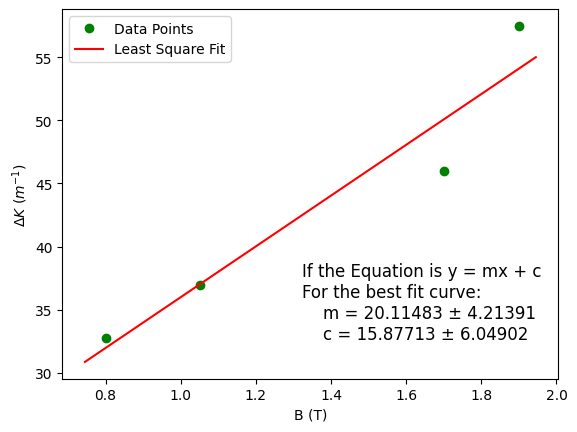
\includegraphics[width=0.8\columnwidth]{graph.png}
		\caption{$\Delta K$ vs $B$ graph}
		% \caption{\textbf{Splitting of lines in cadmium}}
		\label{fig:graph}
	\end{figure}
\subsection{Error Calculation}

    $$\Delta \mu_B = \mu_B \frac{\Delta slope}{slope} = \mu_B \times \frac{4.214}{20.115}$$

    $$\Delta \mu_B = 8.3 \times 10^{-25} Am^2$$